%----------------------------------------------------------------------------------------
%        PACKAGES AND OTHER DOCUMENT CONFIGURATIONS
%----------------------------------------------------------------------------------------
\documentclass[Coupling]{../../data/TelemacDoc} % Default font size and left-justified equations
%\documentclass[Telemac2D,french]{TelemacDoc} % Default font size and left-justified equations in french

\usepackage{verbatim}
\usepackage[toc,page]{appendix} 
\usepackage{fancyhdr}
\usepackage{color}
\usepackage{url}

\begin{document}

\let\cleardoublepage\clearpage

\title{Mascaret - Telemac2D\\longitudinal coupling}
\subtitle{User Manual}
\version{\telmaversion}
\date{\today}
\maketitle
\clearpage

\newpage
\thispagestyle{empty}
\TelemacCopyright{}

\pagestyle{empty}
\tableofcontents

\pagestyle{fancy}

\chapter{Introduction}
Several research works have recently been published on the
longitudinal coupling of hydraulic solvers from the Open
Telemac-Mascaret suite. \cite{Tayachi2013}, \cite{Tayachi2014}, and
\cite{PhDDaou} can be cited for example. 
The integrated Mascaret - Telemac2D longitudinal coupling described in
this document is based on S\'ebastien Barth\'el\'emy's post-doc at
CERFACS, under the 
direction of S.~Ricci, N.~Goutal and \'E.~Le Pape, who implemented a
fully working prototype for coupling the 1D and 2D free surface
hydraulics models MASCARET and TELEMAC interfaced at their boundary
conditions, denoted in the following as longitudinal coupling
\cite{Barthelemy2018, BarthelemyPhD,
  Ricci2018EoCoE}. Fig.~\ref{fig:Schema_1D-2D_interface} illustrates
the 1D sub-domains (in black) coupled to the 2D domains (in blue) at
the interfaces (in red). 
\begin{figure}[htbp]
    \centering
        \centering 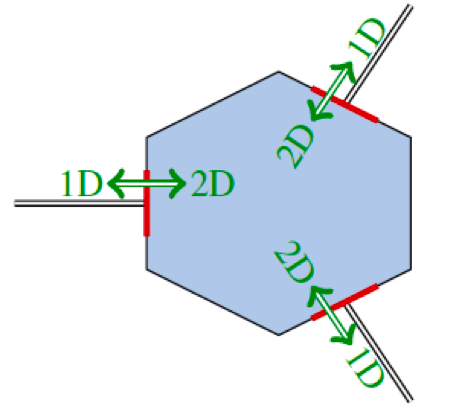
\includegraphics[width=6cm]{figures/Schema_1D-2D_interface.png}
    \caption{Schematic view of longitudinal coupling}\label{fig:Schema_1D-2D_interface}
\end{figure}

The original prototype, based on the article by \cite{Malleron2011},
has been implemented by the explicit coupling 
of two separate F90 codes via the OpenPALM coupler developed at
CERFACS \cite{piacentini2011palm}. The exchanged data was accessed and
modified via the F90 
generic API's of the version 7 of the TELEMAC-MASCARET code suite.

The prototype has been tuned and tested on a single real applicative case
where the confluence of the Nive and the Adour rivers in Bayonne is
modeled with TELEMAC-2D and the upstream Nive and Adour and the
downstream Adour stretches are modeled with MASCARET. For this case
study, three 1D sub-domains are considered: two 1D sud-domains
represent the Nive and Adour rivers (respectively Adour upstream and
Nive upstream) that gather in the 2D domain, then the Adour river is
represented by a downstream 1D model (Adour downstream) as illustrated
in Fig.~\ref{fig:schema_coupling_2}. 
\begin{figure}[htbp]
    \centering
        \centering 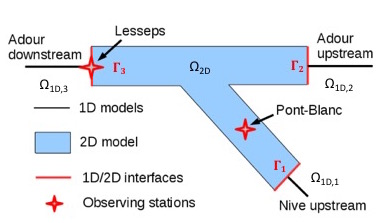
\includegraphics[width=10cm]{figures/schema_coupling_2.jpg}
    \caption{Schematic representation of the relative placement of the
      1D models compared to the 2D model and the coupling interfaces
      for the Adour catchment.}\label{fig:schema_coupling_2} 
\end{figure}

Lately, the code has been rewritten, keeping the same algorithmic
approach, but relying entirely on the python API's and directly
coupling the 1D and 2D components via MPI without any third parties coupler.
An academic test case of hydrodynamics in a 1D rectangular channel was also added for validation with respect to the analytical solution.

At the current state of development, the coupling tools described in
this document allow for the implementation of longitudinal couplings
for configurations similar to the one tested in the prototype: a
single 2D basin with upstream and downstream 1D coupled
stretches. This means that the coupling can handle several 1D
sub-domains and a single 2D sub-domain. 

Note that in such  configuration a coupled 1D stretch
can only have a single interface with the 2D region. This limitation
could be overcome in order to allow for 2D-1D-2D configurations:
the formalism for the description of the 
coupling geometry is already well adapted to complex configurations.\newline

In the following, we'll quickly recall the algorithmic principles,
we'll provide a quick start installation guide (with details in
appendix) and user guide and we'll explain thoroughly the syntax of
the python dictionaries (optionaly stored in json files) used to
describe the coupling configuration and the 
current run definition.

\chapter{The algorithm}\label{algo}

The longitudinal coupling is dealt with via the Schwarz 
algorithm in its multiplicative or additive variants. It will be
illustrated here on the case of a 1D stretch 
upstream of a 2D region as shown in
Fig.~\ref{fig:interface_1D_2D}. The flow in the 1D region is assumed
to be sub-critical (for further considerations on the most adapted
interface 
conditions accordingly to the flow regime, the reader can refer to
[Goutal. HDR]).
\begin{figure}[htbp]
    \centering
    \includegraphics[width=8cm]{figures/interface_1D_2D.png}
    \caption{Schematic representation of the relative placement of the
      1D models compared to the 2D model on a simple 1D-2D
      configuration.}\label{fig:interface_1D_2D} 
\end{figure}

The Schwarz method is an iterative algorithm illustrated in
Fig.~\ref{fig:schemacoupling_time1}: the time range of the coupling
event is split into a sequence of time intervals, as in $[t_1, t_2]$. The
iterations in a given interval are represented by the red loop.
Over each interval,
models (code A and code B) are integrated in time, with their
respective time steps. It should be noted that one code could be
faster then the other, and thus would have to wait before exchanging
data. Once both models have computed their hydraulic states, they
exchange (via communications denoted by com) some hydraulic state
variables
-- here the free surface
height and the discharge values --
at the boundary of the 1D and 2D sub-domains, until a convergence criteria is
reached. In case of a sub-critical flow, the upstream 1D model
provides the discharge boundary condition value to the 2D model which,
in turns, provides the 1D with the free surface height condition. On
the same time interval, the models are therefore restarted and
integrated with the new boundary conditions. This is referred to as a
{\em coupling step}. Once the convergence (or the maximum number of allowed 
iterates) is reached, the models are integrated on the following time
interval, for the next coupling step. The coupling steps are chained
to cover the entire coupling event. 
\begin{figure}[htbp]
    \centering
    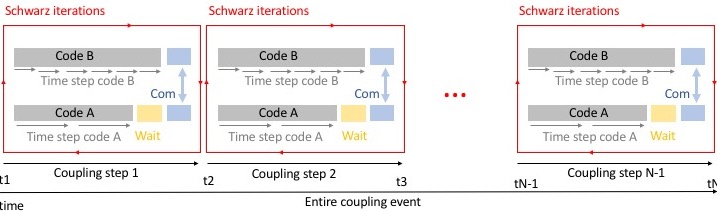
\includegraphics[width=12cm]{figures/schemacoupling_time1.jpeg}
    \caption{Schema}\label{fig:schemacoupling_time1}
\end{figure}

The Schwarz method is derived in a multiplicative or additive variant
depending on how time is dealt with during the iterative process at
the coupling interfaces $\Gamma$. 

In the \emph{multiplicative} variant, the models are integrated one at a
time in a sequence, starting in the present study with the 1D
model. As a consequence, only the 1D model restarts from initially 
prescribed boundary conditions at the coupling interfaces or from
conditions inherited from the previous time interval as in
Eq.~\ref{eq:schwarz_1D_model}. The 2D model 
always runs after at least a 1D integration, therefore the boundary
conditions at the coupling interfaces are always provided by the 1D
model as in Eq.~\ref{eq:schwarz_2D_model_multi}.
\begin{equation}
\left\lbrace
\begin{array}{l}
\mathcal{L}_1 (S,Q)^k = 0 \textrm{ on } \Omega_{1D} \times [t_1;t_2] \\
S_{1D}^k = A_{21}(\bar{h}_{2D}^{k-1}) \textrm{ on } \Gamma \times [t_1;t_2] \\
\end{array}
\right.
\label{eq:schwarz_1D_model}
\end{equation}

\begin{equation}
\left\lbrace
\begin{array}{l}
\mathcal{L}_2 (h,u,v)^{k} = 0 \textrm{ on } \Omega_{2D} \times [t_1;t_2]\\
(u,v)_{2D}^{k} = B_{12}(Q^{k}_{1D}) \textrm{ on } \Gamma \times [t_1;t_2] \\
\end{array}
\right.
\label{eq:schwarz_2D_model_multi}
\end{equation}

\begin{equation}
\left\lbrace
\begin{array}{l}
\mathcal{L}_2 (h,u,v)^{k} = 0 \textrm{ on } \Omega_{2D} \times [t_1;t_2]\\
(u,v)_{2D}^{k} = B_{12}(Q^{k-1}_{1D}) \textrm{ on } \Gamma \times [t_1;t_2] \\
\end{array}
\right.
\label{eq:schwarz_2D_model_add}
\end{equation}

In the \emph{additive} variant, the models are integrated simultaneously:
both restart from initially prescribed boundary conditions at the
coupling interfaces or from conditions inherited from the 
previous time interval as in Eq.~\ref{eq:schwarz_1D_model} and
Eq.~\ref{eq:schwarz_2D_model_add}. The additive variant is available
as an option because it has the advantage that the models can run 
simultaneously in parallel, but it has to be noted that in some
situations the additive formulation has a slower convergence than the
multiplicative formulation, and, even if the models run in
parallel, the overall coupling time could be higher than with the
multiplicative variant. The default choice is therefore the
multiplicative Schwarz method.


\begin{figure}[htbp]
    \centering
        \centering 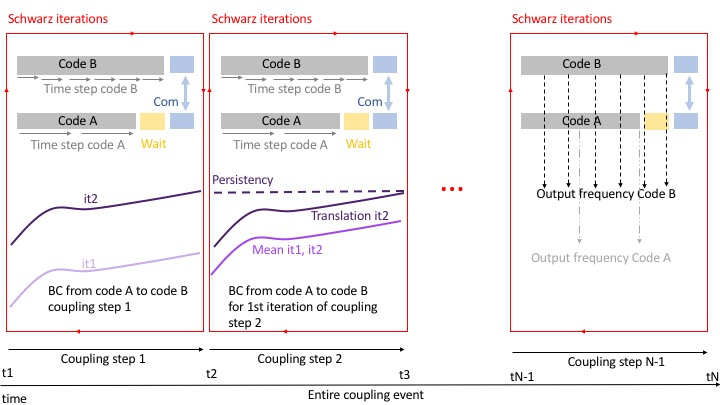
\includegraphics[width=12cm]{figures/schemacoupling_time2.jpeg}
    \caption{Schematic representation of the coupling with coupling step sequneces.}\label{fig:schemacoupling_time2}
\end{figure}
The algorithm is also described by the way boundary
conditions at the interface are inherited from the previous to the
current coupling step as illustrated in Fig.~\ref{fig:schemacoupling_time2}. A
possible choice is to reuse the same
conditions as in the \emph{previous} time interval. If the time
interval spans more than one model time-step, the whole time series is
translated to the next interval. An alternative is to make the last
value of the time series \emph{persist} as a constant on the following
interval. A further distinction, especially if the iterates are stopped
before satisfactory convergence, is to use the last value at the
boundary as it has been provided by the other model before the last
integration or as it has been updated by the model itself after the last
integration. The default choice is the persistence of the last value
provided by the other model.

In order to cope with the oscillation in values during iterates before
convergence, the average of the values (or time series) from the last
two iterates is used instead of the last value itself. This
approximation could be avoided if the algorithm is iterated till full
convergence. 

\chapter{Software requirements and installation}

The longitudinal coupling has been implemented on top of the version
8.1 of Open TELEMAC-MASCARET, provided with the recently updated
python3 API's. In addition, some specific python3 procedures have been
added for the coupling.
\newline

In order to have a coherent complete python3 environment with all
the needed packages, we suggest creating a
dedicated environment either via a python3 venv -- as illustrated in
appendix \ref{ann:venv_install} -- or miniconda -- as illustrated in
appendix \ref{ann:conda_install}. 
\newline

The Open TELEMAC-MASCARET code has to be compiled with the ``api''
target activated. Since the coupling needs the message passing MPI
library, choose a compilation environment with its own compatible MPI
library, even if TELEMAC2D will be used in its sequential
declination. Notice and remember that the python environment will
include \texttt{mpi4py} and some caution has to be paid to be sure
that the underlying MPI library is the same as that for the model. More
details are provided in sections
\ref{ann:venv_mpi4py} and \ref{ann:mpi4py} of the
appendix on the venv and conda installations.
\newline

Once the environment has been created and loaded, you can
proceed to the compilation of the models with the python3 utility
\texttt{scripts/python3/compile\_telemac.py}. Please refer to the Open
TELEMAC-MASCARET documentation for details.

Note that the configuration for the
longitudinal coupling in \texttt{configs} must contain the following
informations (examples here refer to gfortran and OpenMPI4, please
modify the syntax 
accordingly to your compiler)
\begin{verbatim}
options:     mpi api
f2py_name: f2py
pyd_fcompiler: gfortran
sfx_lib:    .so
cmd_obj:    mpif90 -c -cpp -fPIC [...]
cmd_lib:    mpif90 -fPIC -shared [...]
cmd_exe:    mpif90 -fPIC [...]
cmd_obj_c: mpicc -c -fPIC <srcName> -o <objName>
cmd_obj_partel: mpif90 -c -cpp -fPIC [...]
mpi_cmdexec: mpirun [...] -np <ncsize> <exename>
\end{verbatim}

Finally, make sure that the python modules are made accessible for
import, by adding the \texttt{\$HOMETEL/scripts/python3} directory to
the \texttt{PYTHONPATH} environment variable. 

\chapter{Naming conventions}\label{namcon}
In order to be consistent throughout the document, we point out
in this chapter some naming conventions and keywords we'll use in
the following.

\section{Time reference and cycling}\label{namcon:TIMECYCLE}
A coupled simulation is a time evolving prognostic model used to
simulate a multi-physics phenomenon. The simulation implies different
specialized models that cooperate to represent a complex system. All
models must reference the same physical simulated situation,
therefore it is mandatory to define a common time reference.

Furthermore a complex system on a long event could not be
simulated in a single integration, neither it is safe to perform such
integration without restarting capabilities. For this reason the
coupled simulation is implemented by cycling runs as
illustrated in Fig.~\ref{fig:schemacoupling_time3} and detailed in the following section.

\begin{figure}[htbp]
    \centering
        \centering 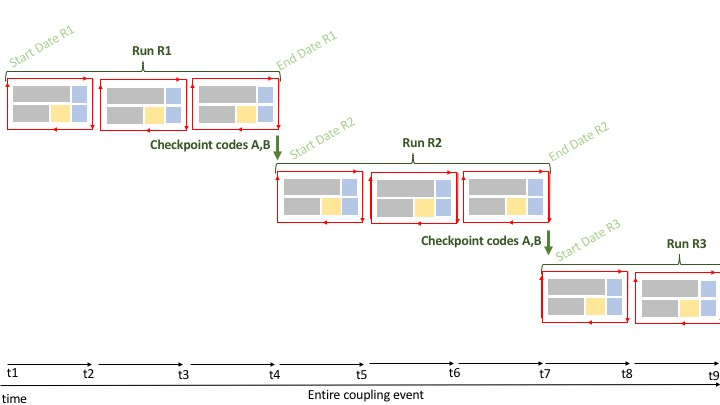
\includegraphics[width=12cm]{figures/schemacoupling_time3.jpeg}
    \caption{Schematic representation of coupling with sequential runs  }\label{fig:schemacoupling_time3}
\end{figure}

All time instances are referenced as {\bf elapsed seconds}
from a common {\bf reference date}. The elapsed seconds are the common unit, and as such, are used in files
and directories names. Yet, in the configuration files, human readable
dates are used and automatically converted into 
elapsed seconds by the coupling scripts. The reference date is the initial instant of an
{\bf event} and the simulation cannot start before that date. 

A {\bf run} denotes a coupled simulation over a sub period 
of the event. It is defined by a {\bf start date} (which
should be greater or equal than the reference date) and an
{\bf end date} (which should be strictly greater than the
start date). Restarting capabilities allow for chaining a subsequent
run starting from the previous end date. Yet a cold start is possible, provided that initial conditions for each
model are available at the start date. A {\em run} is either 
{\bf restarted from a file containing a
previously saved information}, or if {\em initialized from provided conditions at the beginning of the event}.  
Each run can be subdivided into a sequence of chained shorter
{\bf executions} of a prescribed {\bf duration}, for the
purpose of reducing the resources needed for every single parallel
application and of generating frequent {\bf checkpoints}  to
increase fault resiliency. 
\newline

For illustration purposes, the time line in Fig.~\ref{fig:schemacoupling_time3} is detailed here:

A 1-month {\em event} is considered, starting at midnight of July the 1st
2019. The {\em reference date} is therefore \texttt{1/7/2019
  00:00:00}.

In order simulate the 6-hour interval from noon to 7 pm of the same day,
the {\em run} is defined with {\em start date} \texttt{1/7/2019
  12:00:00} and {\em end date} \texttt{1/7/2019 18:00:00}, provided
that at least the initial conditions for all the models are available
at the start date, for instance  $t_1$ to $t_7$ in Fig.~\ref{fig:schemacoupling_time3}.

The run could also be slit the run into 2 checkpointed executions of 3
hours each with {\em  execution duration} of
\texttt{03:00:00} between $t_1$ and $t_4$ and then between $t_4$ and $t_7$.

In order to pursue the simulation for 3 more hours, a {\em
  new run} is defined with {\em start date} \texttt{1/7/2019
  18:00:00} and {\em end date} \texttt{1/7/2019 21:00:00} strating 
the restart produced by the previous run at $t_7$.

\section{Coupling definition}\label{namcon:COUPLING}
The main algorithmic concepts are described in chapter \ref{algo}. We
draw here some correspondences between the algorithm and naming
 used in the configuration dictionaries or files, relying
on Fig.~\ref{fig:schemacoupling_time1},
Fig.~\ref{fig:schemacoupling_time2} and
Fig.~\ref{fig:schemacoupling_time3}. 

The toplevel choice, referencing to the multiplicative and
additive variants of the Schwarz formulation, is the {\bf coupling
  method}.
\newline

Successively, a coupled simulation is realised
as a time sequence of {\bf coupling steps}. The step is the {\em coupling time interval}
mentioned in chapter~\ref{algo}, i.e. the frequency at which the
boundary conditions are recomputed and exchanged till convergence. A
short coupling step makes the convergence easier, a longer time step
reduces the overall number of repetitions but could require more
iterates per repetition. In order to control the execution time and
prevent hanging execution in case of divergence, the
iterative process is bounded to a prescribed {\bf maximum number of iterates}.
\newline

\section{1D models description}\label{namcon:1DMOD}
The coupling framework relies on a hydraulic network that features at least one 1D stretch modeled with
Mascaret.  Each 1D domain is identified with a unique {\bf identifier} string.
\newline

The {\bf time step} is indicated for each model; it must
divide exactly the {\em coupling step}. Note that, in the
current version of the coupling scripts, all 1D models share the same time step while the 2D model has its own time step.
The need for distinct 1D model time steops will be further evaluated. 
\newline

The paths for Mascaret input and output files should be given,
as detailled in section \ref{ftree:MASCARET}. The information is stored 
in a disctionary (optionally in a json file) for each
1D model. 

\section{2D model description}\label{namcon:2DMOD}
Whether the representation of non contiguous 2D
domains should be treated with separate instances of Telemac
or with a single instance with a non contiguous computational
domain is still open for discussion. Most likely, a single instance would be used, nevertheless, in
order to maintain the two options, the 2D model
is also identified with a unique {\bf identifier} string.  
Similarly to the 1D model, the 2D model {\bf time
  step} must be prescribed and divide exactly the {\em coupling step}.

The {\bf output frequency}, at which the
model writes its results in the output files, and the {\bf output
  location}, for nodes of interest should be specified.
  
Path for Telemac input and output files should also be given,
as detailled in section \ref{ftree:TELEMAC2D}, in the form of a dictionnary (optionnaly in a json file).
%ascii version is still supported to make the porting of existing
%configurations easier. 

\section{Interfaces description}\label{namcon:INTERF}
Interfaces description explains how the models are connected.  
For the longitudinal coupling, there is no overlapping between 1D and 2D domains. The coupling interfaces are located 
at the extremities of 1D stretches and free boundaries of the 2D
domain as shown in Fig.~\ref{fig:schema_coupling_2}.

An {\bf interface} $\Gamma$ is fully described by the {\bf
  identifier of the 1D model}, the {\bf identifier of the 1D stretch
free extremity} coupled to the 2D model, the {\bf
  identifier of the 2D model}, the {\bf identifier of the 2D liquid
boundary} coupled to the 1D model, and by the {\bf relative position
  of the 1D model} w.r.t. the 2D model (upstream or downstream).
\newline

The iterative coupling process described in Sect.~\ref{algo} is
stopped when specific {\bf convergence criteria} at the interfaces are
met. For each interface, the coupled variables and the convergence threshold should be specified. 

\chapter{Inputs for a coupled application}\label{ftree}
A coupled application is based on a set of MASCARET and
TELEMAC2D instances along with the description of the simulation (Section
\ref{namcon:TIMECYCLE}) and the coupling configuration. 
\newline

The \texttt{LongCplDriver} class from \texttt{telapy.coupling.long\_cpl\_driver} drives a coupled
application. It receives its inputs via dictionaries. 
Arguments for initialisation of the \texttt{LongCplDriver} class are:
\begin{itemize}
\item[$\bullet$] The directory path \texttt{caseo\_path} for toplevel of the coupling filetree, naled \texttt{CPLROOT in the following}, 
\item[$\bullet$] A dictionnary \texttt{coupling\_def} for coupling information (Sect.~\ref{json:CouplingDef}),
\item[$\bullet$] A dictionnary \texttt{model\_configs} for 1D and 2D models information, espacially path for input files for the 1D and 2D submodels (Sect.~\ref{ftree:MASCARET} and Sect.~\ref{ftree:TELEMAC2D}), 
\item[$\bullet$] A bolean \texttt{keep\_exec} for saving of execution directory \texttt{CPLROOT/EXEC}. Note that this path is the reference for input and output relative paths.
\end{itemize}
Arguments for call of the \texttt{LongCplDriver} class stand in a dictionnary that gathers information on the simulation (Sect.~\ref{json:ConfigRun})

There are two ways to run a coupling. The first way consists in
invoking the driver from a user python procedure that provides the
previously mentionned dictionaries, initialize and call the
\texttt{LongCplDriver} class. The second way relies on a provided
launcher \texttt{run\_cpl.py long} as explained in Chapt.~\ref{running}. In the latter case, the input information is read from configuration files gathered as a dictionnary in a single python file \texttt{coupling\_description.py} 
or in a set of json files with similar dictionnary structure.  
The syntax for the arguments of initialisation and call methods of 
\texttt{LongCplDriver}, as well as how this information is stored in 
in python or json as described in the following subsections. 

The actual input files for 1D and 2D submodels should be available in a remote directory, on a file system accessible for linking from inside \texttt{CPLROOT/EXEC}. 
The output file location \texttt{Results} should be specified (Chap.~\ref{running}), possibly not under the temporary \texttt{CPLROOT/EXEC} directory.

\section{MASCARET}\label{ftree:MASCARET}
\subsection{Description of MASCARET inputs}
A Mascaret 1D instance is described by an xml parameter file
with extension \texttt{.xcas}. The geometry is described
in a geometry file with extension \texttt{.geo}.  
The initial condition for restart is read from an ascii file with extension \texttt{.lig}.
The time varying boundary conditions are described in several
files (one per condition) with extension \texttt{.loi} or \texttt{.law}. The data describing MASCARET input files come as the third argument of \texttt{LongCplDriver} class.  Three posibilities are handled to provide this information to \texttt{LongCplDriver} class: as a dictionnary, in a python file or in a json file.  The checkpointed boundary conditions at the
coupling interfaces are automatically stored in a json file named 
\texttt{bc1D\_restart\_}; indexed by the  model identifier
and seconds since the {\em reference
  date} (e.g. \texttt{bc1D\_restart\_AAM\_57600.json}). These files are 
not provided by the user and are created during the coupling cycles. 
The data describing MASCARET input files come as an element of the third argument of \texttt{LongCplDriver} class given in the \texttt{model\_configs} dictionnary.  Three posibilities are handled to provide this information to \texttt{LongCplDriver} class: as a dictionnary, in a python file or in a json file. 

\subsection{Description of MASCARET input data as a dictionary for \texttt{LongCplDriver}}
The third positional argument of the initialization of
\texttt{LongCplDriver} is a dictionnary named \texttt{models\_configs} that describes the configurations for the 1D and 2D submodel distinguished by their identier as \texttt{"config\_}{\em identifier}\texttt{"}. For instance, if the identifier for the ``Channel 1D'' model is
\texttt{ch1d}, its corresponding key in the dictionnary is \texttt{config\_ch1d}
\newline

Under each of the 1D submodel key, the paths for MASCARET input files are listed in a dictionnary under the single key {\bf\texttt{files}}:
\begin{description}
\item[\texttt{xcas}] string with the path of the xml parameter file
\item[\texttt{geo}] string with the path of the geometry file
\item[\texttt{res}] string with the name (and only the name as the path is set at run time) of the
  results file
\item[\texttt{listing}] string with the name (and only the name, because the path is determined at run time) of the listing file
\item[\texttt{damocle}] only kept for compatibility. Its value is a
  string but the content is neglected
\item[\texttt{lig}] string with the path of the initial condition file. Note that during the coupling process this can be overidden in order to reuse restart.
\item[\texttt{loi}] list of strings with the path of the time dependent boundary condition files.
\end{description}

As an example, if the dictionary to be passed as third argument to
\texttt{LongCplDriver} is stored in \texttt{model\_configs}, the
section for the ``Channel 1D'' model will be as follows:
\begin{verbatim}
models_configs = {
  "config_ch1d" : {
     "files": {

        "xcas": "../Input_Data/1d_stretch/ParametresMascaret.xcas",
        "geo": "../Input_Data/1d_stretch/Channel1d.geo",
        "res": "ResultatsOpthyca_ch1d.opt",
        "listing": "ResultatsListing_ch1d.lis",
        "damocle": "listing.damoc",
        "lig": "../Input_Data/1d_stretch/WaterLine_ch1d.lig",
        "loi": [
                "../Input_Data/1d_stretch/1d_up.loi",
                "../Input_Data/1d_stretch/1d_down.loi"
               ]
     }
  },
  [...]
\end{verbatim}

\subsection{Description of MASCARET input data as an entry in \texttt{coupling\_description.py}}
If the coupling is started by the standalone launcher
\texttt{run\_cpl.py long}, the coupling description can be stored in
a python file with compulsory name \texttt{coupling\_description.py}.  
In this file, for each 1D model instance, a dictionary must be defined and given
the mandatory name\\
\texttt{config\_}{\em identifier}

The dictionaries content is the same as in the dictionary argument described in
the previous section. For instance, the dictionary for the ``Channel 1D'' model is:
\begin{verbatim}
config_ch1d = {
  "files": {

     "xcas": "../Input_Data/1d_stretch/ParametresMascaret.xcas",
     "geo": "../Input_Data/1d_stretch/Channel1d.geo",
     "res": "ResultatsOpthyca_ch1d.opt",
     "listing": "ResultatsListing_ch1d.lis",
     "damocle": "listing.damoc",
     "lig": "../Input_Data/1d_stretch/WaterLine_ch1d.lig",
     "loi": [
             "../Input_Data/1d_stretch/1d_up.loi",
             "../Input_Data/1d_stretch/1d_down.loi"
            ]
          }
}
\end{verbatim}

\subsection{Description of MASCARET input data as a json configuration file }
Another option, if the coupling is started by the standalone launcher
\texttt{run\_cpl.py long}, is to provide a json configuration file 
for each model instance, named \\
\texttt{config\_}{\em identifier}\texttt{.json}.

This json file contains a dictionary with a single key \texttt{files}. For instance, the json configuration file named after the identifier of the ``Channel 1D'' submodel as \texttt{config\_ch1d.json}, contains:
\begin{verbatim}
{
 "files": {
    "xcas": "../Input_Data/1d_stretch/ParametresMascaret.xcas",
    "geo": "../Input_Data/1d_stretch/Channel1d.geo",
    "res": "ResultatsOpthyca_ch1d.opt",
    "listing": "ResultatsListing_ch1d.lis",
    "damocle": "listing.damoc",
    "lig": "../Input_Data/1d_stretch/WaterLine_ch1d.lig",
    "loi": [
            "../Input_Data/1d_stretch/1d_up.loi",
            "../Input_Data/1d_stretch/1d_down.loi"
           ]
    }
}
\end{verbatim}

\section{TELEMAC2D}\label{ftree:TELEMAC2D}
\subsection{Description of TELEMAC2D inputs}
A Telemac 2D instance is described by an ascii parameter file
in the {\em damocles} format, usually called the {\em cas} (french for
case) file. Its extension is usually (but not necessarily) \texttt{.cas}.  
The geometry and the physical characteristics of the domain are
described in a binary file in the {\em selafin} format, with extension
\texttt{.slf}. If the model is restarted, the initial condition has
to be stored in another selafin file with extension \texttt{.slf}.  
The boudary conditions settings are given for the
peripheral grid cells in an ascii file with extension
\texttt{.cli}. When needed, the time varying boundary conditions are stored in
a separate ascii file with extension \texttt{.liq}
\newline

For restarted coupling, the checkpointed boundary conditions at the
coupling interfaces are automatically stored in a json file named adfter the model 
identifier and time in seconds since the {\em reference
  date} as \texttt{bc2D\_restart\_} (for instance \texttt{bc2D\_restart\_Bayonne\_57600.json}). These files are not provided by the user and are created during the executions cycling.

\subsubsection{An important remark about restart file names}
In order to allow for the time cycling described in section
\ref{namcon:TIMECYCLE}, the names of the initial condition files for
the 2D model must respect the mandatory naming convention\\
\texttt{WaterLineInit\_}{\em seconds}\texttt{.slf}\\
where the seconds are computed w.r.t. the common reference date. 
The coupling driver will link the currently selected initial condition
file to the constant name\\
\texttt{WaterLineInit\_in.slf}\\
before transferring it to the execution directory as
\texttt{T2DPRE}. It is therefore recommended to describe the restart
file in the \texttt{.cas} description by\\
\texttt{FICHIER DU CALCUL PRECEDENT = WaterLineInit\_in.slf}\\
or\\
\texttt{PREVIOUS COMPUTATION FILE = WaterLineInit\_in.slf}

\subsection{Description of TELEMAC2D inputs as a dictionary for \texttt{LongCplDriver}}
The third positional argument of the initialization of
\texttt{LongCplDriver} is a dictionnary named \texttt{models\_configs} that describes the configurations for the 1D and 2D submodel distinguished by their identier as \texttt{"config\_}{\em identifier}\texttt{"}. For instance, if the identifier for the ``Channel 2D'' model is
\texttt{ch2d}, its corresponding key in the dictionnary is \texttt{config\_ch2d}.
\newline

Under this key is a dictionnary that gathers the following keys and information:
\begin{description}
\item[\texttt{cas}] string with the path of the case parameter file,
\item[\texttt{config\_file}] Optional: string with the
  path of the systel compilation configuration file. Its default is the content of the
  \texttt{SYSTELCFG} environment variable. The same environment
  variable can be referenced in the dictionary (especially in the json
  files) by the conventional string \texttt{"\$\{SYSTELCFG\}"},
\item[\texttt{config\_option}] Optional: string with the identifier of
  the compilation configuration of the Telemac system. Its default is the content of the
  \texttt{USETELCFG} environment variable. The same environment
  variable can be referenced in the dictionary (especially in the json
  files) by the conventional string \texttt{"\$\{USETELCFG\}"}
\end{description}

As an example, if the dictionary to be passed as third argument to
\texttt{LongCplDriver} is stored in \texttt{model\_configs}, the
section for the ``Channel 2D'' model is:
\begin{verbatim}
models_configs = {
  [...]
  "config_ch2d" : {
     "files": {
        "cas": "../Input_Data/2d_rect/T2DCAS",
        "config_file": "${SYSTELCFG}",
        "config_option": "${USETELCFG}"
     }
  }
}
\end{verbatim}

\subsection{Description of TELEMAC2D inputs as an entry in \texttt{coupling\_description.py}}
If the coupling is started by the standalone launcher
\texttt{run\_cpl.py long}, the coupling description can be stored in
a python file with compulsory name  \texttt{coupling\_description.py}.  In this file, 
for the 2D model, a dictionary must be defined and given the mandatory name
\texttt{config\_}{\em identifier}.

The dictionaries content is the same as in the dictionary argument described in
the previous section. For instance, the dictionary for the ``Channel 2D'' model is:

\begin{verbatim}
config_ch2d = {
  "files": {
     "cas": "../Input_Data/2d_rect/T2DCAS",
      "config_file": "${SYSTELCFG}",
      "config_option": "${USETELCFG}"
  }
}
\end{verbatim}

\subsection{Description of TELEMAC2D inputs as a json configuration file}
Another option, if the coupling is started by the standalone launcher
\texttt{run\_cpl.py long}, is to provide a json configuration file 
for the 2D model, named \\
\texttt{config\_}{\em identifier}\texttt{.json}.

This json file contains a dictionary with a single key \texttt{files}. For instance, the json configuration file named after the identifier of the ``Channel 2D'' submodel as \texttt{config\_ch2d.json}, contains:
\begin{verbatim}
{
 "files": {
    "cas" : "../Input_Data/2d_rect/T2DCAS",
    "config_file": "${SYSTELCFG}",
    "config_option": "${USETELCFG}"
    }
}
\end{verbatim}

\section{The Coupling Definition}\label{json:CouplingDef}
The second argument for initialization of the coupling driver
\texttt{LongCplDriver} class is the \texttt{coupling\_def} dictionary that describes the coupling information.

If the coupling is started by the standalone launcher
\texttt{run\_cpl.py long}, the coupling description is stored in
a python file with the compulsory name of \texttt{coupling\_description.py} stored in
\texttt{CPLROOT} and the coupling definition is stored in a
dictionary with the mandatory name \texttt{coupling\_def}.\\
As an alternative it can be stored in a json in
\texttt{CPLROOT} with the mandatory name\\
\texttt{CouplingDef.json}\\

In detail, the definition is organised in 4 sections, described in the following, and corresponding to
4 toplelvel keys in the the dictionary or separate json
blocks in the json file:
\begin{itemize}
\item\texttt{"Coupling"}
\item\texttt{"1D"}
\item\texttt{"2D"}
\item\texttt{"Interfaces"}
\end{itemize}
Each block contains in turn a dictionary.  A full example is provided in Appendix \ref{app:coupling_description}
or \ref{app:driven_coupling} or \ref{app:CouplingDef}

\subsection{The \texttt{Coupling} entry}
The \texttt{Coupling} entry contains the following keys ({\em cf.} \ref{namcon:COUPLING}):
\begin{description}
  \item[\texttt{TimeStep}] the value is a real number with the
    coupling step in seconds    
  \item[\texttt{Method}] the value is a string. The choice is limited to
    \texttt{MultiplicativeSchwarz} or\\
    \texttt{AdditiveSchwarz}
  \item[\texttt{MaxIter}] the value is an integer with the maximum
    number of iterates allowed per coupling step
  \item[\texttt{CplStepRestart1D}] (optional, defaulting to
    \texttt{Persist2D}) the value is a string indicating how to
    reinitialize the 1D boundary conditions at coupling interfaces at
    each new coupling step
  \item[\texttt{CplStepRestart2D}] (optional, defaulting to
    \texttt{Persist1D} and relevant only for the additive variant of
    the Schwarz method) the value is a string indicating how to
    reinitialize the 2D boundary conditions at coupling interfaces at
    each new coupling step
\end{description}

\subsection{The \texttt{1D} entry}
The \texttt{1D} entry contains as many dictionaries as instances of the 1D
model. Each dictionary uses as key the identifier of the 1D model ({\em
  cf.} \ref{namcon:1DMOD}) and contains two keys:
\begin{description}
  \item[\texttt{TimeStep}] the value is a real number with the
    timestep for the model integration in seconds. Remember that, in the 
    current version, the time step has to be the same for all the 1D 
    models   
  \item[\texttt{OutputFreq}] the value is a real number with the
    results output frequency in seconds
\end{description}
 
\subsection{The \texttt{2D} entry}
The \texttt{2D} entry contains as many dictionaries as instances of the 2D
model (only one possible as of today) and contains three keys: 
\begin{description}
  \item[\texttt{TimeStep}] the value is a real number with the
    timestep for the model integration in seconds.
  \item[\texttt{OutputFreq}] the value is a real number with the
    results output frequency in seconds
  \item[\texttt{OutputSites}] the value is a list of integers with the
    node number at which the resulsts are output. Note that also for a
    single point the list syntax \texttt{[32939]} has to be respected
\end{description}

\subsection{The \texttt{Interfaces} entry}
The \texttt{Interfaces} entry is a list of dictionaries.  
Each dictionary describes a single coupling interface ({\em cf.}
\ref{namcon:INTERF}) and contains the following keys:
\begin{description}
  \item[\texttt{Id1D}] the value is a string with the identifier of
    the 1D model
  \item[\texttt{IdExtr1D}] the value is a string with the identifier of
    the 1D model coupling free extremity as it is listed in the xml
    \texttt{.xcas} file
  \item[\texttt{Condition1D}] the value is a string with the kind of
    boundary condition at the coupling interface for the 1D model. The
    choice is limited to \texttt{Discharge} or \texttt{WaterLevel}
  \item[\texttt{Id2D}] the value is a string with the identifier of
    the 2D model
  \item[\texttt{LiqBdry2D}] the value is an integer with the number of
    the 2D model coupling liquid boundary as it is listed in the damocles
    {\em cas} file
  \item[\texttt{1DPosition}] the value is a string with the relative
    position of the 1D model w.r.t the 2D model. The
    choice is limited to \texttt{UpStream} or \texttt{DownStream}
  \item[\texttt{ConvCriteria}] the value is a dictionary with as many
    keys as variables to be checked. For each key the value is a real
    number indicating the convergence threshold for that
    variable. Currently possible keys are \texttt{Height} or \texttt{Velocity}
\end{description}

 
\section{The Current Run Configuration}\label{json:ConfigRun}
In order to describe the simulation for the current run, the user must provide every
run call of an instance of the coupling driver \texttt{LongCplDriver}
with the information listed in Sect.~\ref{namcon:TIMECYCLE}.
The first and only for a run call to an instance of
\texttt{LongCplDriver}, the information has to be
organised in a python dictionary, named \texttt{config\_run}.\\

If the coupling is started by the standalone launcher
\texttt{run\_cpl.py long}, the coupling description is stored in
a python file with the compulsory name of \texttt{coupling\_description.py} stored in
\texttt{CPLROOT} and the coupling definition is stored in a
dictionary with the mandatory name \texttt{config\_run}.\\
As an alternative it can be stored in a json in
\texttt{CPLROOT} with the mandatory name\\
\texttt{ConfigRun.json}. The configuration is organised in 2 sections, corresponding
to two toplelvel keys in the dictionary or two separate json
blocks in the json file:
\begin{itemize}
\item\texttt{"Run"}
\item\texttt{"2D"}
\end{itemize}

Each of them contains in turn a dictionary. A full example is provided in Appendix  \ref{app:coupling_description}
or \ref{app:driven_coupling} or \ref{app:ConfigRun}

\subsection{The \texttt{Run} entry}
The \texttt{Run} entry contains the following keys ({\em cf.} \ref{namcon:TIMECYCLE}):
\begin{description}
  \item[\texttt{RefDate}] the value is a string in the format
    \texttt{[{\em d}]{\em d}/[{\em m}]{\em m}/{\em yyyy} {\em hh}:{\em
        mm}:{\em ss}} with the {\em event} reference 
    date used as origin for the time counters in seconds
  \item[\texttt{StartDate}] the value is a string in the format
    \texttt{[{\em d}]{\em d}/[{\em m}]{\em m}/{\em yyyy} {\em hh}:{\em
        mm}:{\em ss}} with the {\em start date} for the 
    current {\em run}
  \item[\texttt{EndDate}] the value is a string in the format
    \texttt{[{\em d}]{\em d}/[{\em m}]{\em m}/{\em yyyy} {\em hh}:{\em
        mm}:{\em ss}} with the {\em end date} for the 
    current {\em run}
  \item[\texttt{SingleExecDuration}] the value is a string in the format
    \texttt{[{\em dd} day[s]] {\em hh}:{\em mm}:{\em ss}} or
    \texttt{[{\em dd}d][{\em hh}h][{\em mm}m][{\em ss}s]} with the
    duration of every {\em single execution} 
    splitting the current {\em run}. Valid equivalent examples are
    \texttt{"36:00:00"} or \texttt{"1 day 12:00:00"} or \texttt{"36h"}
    or \texttt{"1d12h"}. Notice that this field is optional: if
    missing, the whole run is performed with just one execution. 
  \item[\texttt{RestartFromFile}] the value is the string \texttt{yes}
    or \texttt{no} to indicate if the run restarts from previously
    stored conditions (if available) or if it is a cold start   
  \item[\texttt{SaveCheckPoints}] the value is the \texttt{yes} or
    \texttt{no} string indicating if the restart information have to
    be stored between every single execution (yes) or only at the end
    of the run (no)
\end{description}


\subsection{The \texttt{2D} entry}
The \texttt{2D} entry contains as many dictionaries as instances of the 2D
model (only one possible as of today) and contains two keys: 
\begin{description}
  \item[\texttt{Parallel}] the value is the \texttt{yes} or
    \texttt{no} string indicating if we run the parallel (yes) or the
    sequential (no) telemac2d executable, 
  \item[\texttt{NbProc}] the value is an integer, relevant only if the
    run is parallel, with the number of processors for the 2D model.
\end{description}


\chapter{Running a coupling}\label{running}
Once the input filetree has been prepared and the configuration
dictionaries fully filled, running a coupled application is quite
straightforward.\\

The coupling can be driven from a user application if the\\
\texttt{LongCplDriver} class is imported from
\texttt{telapy.coupling.long\_cpl\_driver}

In such case the coupling definition and model description
information described in the previous sections is 
passed by arguments to the initialization of an instance of the
\texttt{LongCplDriver} class:
\begin{verbatim}
[...]
from telapy.coupling.long_cpl_driver import LongCplDriver
[...]
the_coupling = LongCplDriver(case_path = ".", 
                             coupling_def = user_coupling,
                             models_configs = models_configs)
\end{verbatim}
A fourth optional boolean argument to the initialization, named
\texttt{keep\_exec} allows to conserve the \texttt{EXEC} directory after
deletion of the driver instance or at the end of the procedure, for
debugging purposes. The default is \texttt{keep\_exec=False} and the \texttt{EXEC} directory
is removed.\\

The coupling is actually launched by a direct call of the
\texttt{LongCplDriver} instance which receives the current run
configuration by argument, as in the following example:
\begin{verbatim}
[...]
the_coupling(config_run = driven_run)
\end{verbatim}

More than one run can be chained in the same application, provided
that the \texttt{config\_run} dates are correctly updated as
illustrated in the example in Sect.~\ref{exe:channel_manning} and
appendix \ref{app:driven_coupling}.
$~$\\

The coupling can also be started as a standalone application with the
python procedure\\
\texttt{run\_cpl.py long}\\
provided in the \texttt{scripts/python3/coupling} directory of the 
distributed sources.
\newline

If the procedure is started from the \texttt{CPLROOT}
directory, where the \texttt{coupling\_description.py} -- or the \texttt{CouplingDef.json} and the
\texttt{CurrentRun.json} -- files are, it can be started without any
argument.

If it is started from a generic directory, the \texttt{CPLROOT} has to
be passed as an argument of the \texttt{$--$src} option.
\newline

As an example, for the \texttt{bayonne} test case from the
distribution, let's say that\\
\texttt{CPLROOT} is \texttt{\$HOMETEL/examples/python3/telapy\_coupling/bayonne}\\
while
\texttt{run\_cpl.py long} is in
\texttt{\$HOMETEL/scripts/python3/coupling}

The run can be started from within \texttt{CPLROOT} by
\begin{verbatim}
python $HOMETEL/scripts/python3/run_cpl.py long
\end{verbatim}
or from whatever directory by
\begin{verbatim}
python $HOMETEL/scripts/python3/coupling/run_cpl.py long \
       --src $HOMETEL/examples/python3/telapy_coupling/bayonne
\end{verbatim}

%The option \texttt{$--$keep-exec} allows for conserving the
%\texttt{EXEC} directory after the end of the procedure, for
%debugging purposes. The default is to erase the \texttt{EXEC} directory.
%$~$\\

A summary of the loaded configuration is output
\begin{verbatim}
+--------------------------------------------------------+
|------- LONGITUDINAL MASCARET TELEMAC2D COUPLING -------|
+--------------------------------------------------------+
|
|  Coupling Method: MultiplicativeSchwarz
|  Max It. nr.:     5
|  Coupling TStep:  8.0
|
|  Initial time:    1/7/2019 12:00:00
|  End time:        1/7/2019 16:00:00
|  Split Run every: 02:00:00 (2 exec[s])
|  Restarted run:   yes
|
|  1D models:       ['AAM', 'AAV', 'NA']
|  2D models:       ['Bayonne']
|
|  Interfaces:
|    AAM:limite2  (Discharge ) UpStream   of Bayonne:2
|    AAV:limite1  (WaterLevel) DownStream of Bayonne:3
|    NA:limite2   (Discharge ) UpStream   of Bayonne:1
+--------------------------------------------------------+
\end{verbatim}

The executions start and a progress counter is displayed
\begin{verbatim}
~~~~~~~~~~~~~~~~~~~~~~~~~~~~~~~~~~~~~~
~~~~~   RUN THE COUPLED MODEL    ~~~~~
~~~~~~~~~~~~~~~~~~~~~~~~~~~~~~~~~~~~~~

Running the coupled model between init time 43200 and end time 50400
[====================] 100%

Running the coupled model between init time 50400 and end time 57600
[===============     ]  75%
\end{verbatim}


When the run ends the overall elapsed time is shown
\begin{verbatim}
My work is done. Coupled job lasted : 81.89077615737915 s
\end{verbatim}

\chapter{The Results directory}
After every single execution completes, a subdirectory is created in
\texttt{\$CPLROOT/Results} (Note that the \texttt{Results} directory
is created if not already present). The subdirectory is
indexed by the initial time of the single execution:
\texttt{COUPLING\_FROM\_XXXX}, where \texttt{XXXX} stands for the
number of seconds from the event reference date to the execution
initial time.
\newline

Each subdirectory contains:
\begin{itemize}
\item[$\bullet$] the standard output of the simulation redirected into
  a file named after the {\em cas} configuration file for
  Telemac2D with an additional suffix \texttt{.stdout}  
\item[$\bullet$] the single models results files in the
format of Opthyca files for MASCARET and Selafin files for TELEMAC2D
at the output frequencies entered in the respective sections of the
\texttt{coupling\_def} dictionary or
\texttt{CouplingDef.json} file. (Note that only the results after
the iterative process has converged or reached the maximum number of
iterates are output in these files)
\item[$\bullet$] the convergence criteria files ({\em cf.}
  sect. \ref{res:CONVCRIT}) in human readable ascii or in comma
  separated value (\texttt{.csv}) format to be imported in a spreadsheet
\end{itemize}

Some other output files are stored directly in the input directories
because they are used for restarting the computation. The 1D
waterlines, the 2D state, the boundary conditions for the 1D and the
2D models are stored at the end of every execution if the
checkpointing is activated and, in any case, at the end of the run.

\section{The \texttt{Convergence\_criteria} files}\label{res:CONVCRIT}
At every coupling step, when the iterative process converges or
reaches the maximum number of iterations, six convergence criteria are
computed.

In the \texttt{Convergence\_criteria.out} file (and in its comma
separated value counterpart) at the end of every coupling step, the
effective number of iterates is printed together with the six quantities
evaluated on the 1D and on the 2D (spatial average) side of each
interface.

The quantities are:
\begin{description}
\item[Velocity] symbolized by \texttt{V} computed as $Q/(S1+S2)$
\item[Wetted Area] symbolized by \texttt{SM} computed as $S1+S2$ where
  $S1$ is the main channel wetted area and $S2$ is the floodplain
  wetted area
\item[Discharge] symbolized by \texttt{Q} 
\item[Height] symbolized by \texttt{H} computed as $Z-ZREF$ i.e. the
  water level minus the reference level
\item[First invariant] symbolized by \texttt{I} computed as $Q/(S1+S2)+2\sqrt{g(Z-ZREF)}$
\item[Second invariant] symbolized by \texttt{J} computed as $Q/(S1+S2)-2\sqrt{g(Z-ZREF)}$
\end{description}

\chapter{Examples and validation test cases}

Four test cases are provided in order to illustrate the differents
ways of describing and running a coupling. Moreover these test cases
are run as part of the telemac validation procedure under the tag
\texttt{coupling}:\\
\texttt{python validate\_telemac.py $--$tags coupling}\\

Three tests are implemented a rectangular channel, partly modelled in 1D,
partly in 2D as shown in Fig.~\ref{fig:interface_1D_2D}. The last case
represents the Adour catchment displayed 
in Fig.~\ref{fig:schema_coupling_2}.  

\section{Rectangular channel test case}

\subsection{Description of the test case and experiment settings}

The rectangular channel test case describes a 100 m wide channel
modelled over 10 km with a bathymetry from 5 m upstream to 0
downstream and thus a uniform slope $I = 5.10^{-4}$.  

From the Manning equation, in a permanent regime and with a
homogeneous friction coefficient, the free surface at the equilibrium
is parallel to the bathymetry. Imposing a friction coefficient of
30.6, an upstream inflow $Q=1000 m^3/s$, and a downstream boundary
condition (BC) $Z=5 m$, the analytical solution is $h=5 m$ everywhere,
with a resulting free surface $Z$ ranging from 10 m upstream to 5 m
downstream.  

The hydrodynamics of the channel is modelled with a 5km long 1D model
upstream of a 2D model for the 5 downstream kilometers. There is thus
a unique coupling 1D-2D interface between the 1D downstream BC and the
2D upstream liquid boundary. 

In permanent regime, the 1D-2D coupled solution can be validated
against the analytical solution. 

We design three different experiment settings modifying the initial
conditions (IC) or the upstream inflow boundary condition:   
\begin{itemize}
\item R1: Constant Upstream and downstream BC, 1D and 2D IC already
  set to Manning equilibrium. The solution should remain identical to
  the IC, proving that the coupling does not degrade the permanent
  solution. 
\item R2: Constant Upstream and downstream BC, 1D IC to Manning
  equilibrium, 2D IC set to a horizontal free surface $Z = 8.5 m$ at
  rest. The solution should converge towards the Manning equilibrium
  after a sufficiently long integration, proving that the coupling is
  able to reconstruct the global solution even with non coherent
  initial conditions and a misfit of 1 m on $Z$ and 2 m/s on $V$ at
  the coupling interface. Note that, since the downstream BC
  condition limits $Z$ at the exit, this situation takes longer to
  reach the equilibrium than if the 2D initial condition were lower
  than the analytical value of 7.5 m.  
\item R3: Varying Upstream BC, 1D and 2D IC to Manning equilibrium. In
  this last case, the model starts from the Manning equilibrium, then
  the prescribed upstream inflow is perturbed for 15 minutes, doubling
  the equilibrium value, then dicreases to the original value. The
  Manning equilibrium is temporary lost, but eventually recovered,
  proving that perturbations are correctly propagated throughout the
  coupled models without spurious effects. 
\end{itemize}

\subsection{Test case directory}

The test case files are in 
\begin{itemize}
\item \texttt{examples/python3/telapy\_coupling/channel\_manning} for
  the equilibrium experimental setting (R1),  
\item \texttt{examples/python3/telapy\_coupling/channel\_ic} for the
  equilibrium experimental setting with perturbed initial condition
  (R2),  
\item \texttt{examples/python3/telapy\_coupling/channel\_bc} for non
  permanent experimental setting with perturbed upstream boundary
  condition (R3),  
\end{itemize}

The 1D and 2D model input files are organized as follows : 
\begin{itemize}
\item \texttt{/Input\_Data/1d\_stretch} for the 1D model MASCARET,
  containing the \texttt{.geo}, \texttt{.xcas}, \texttt{.loi} and
  \texttt{.lig} files for geometry, parameters, BC and IC
  respectively. 
\item \texttt{/Input\_Data/2d\_rect} for the 2D model TELEMAC,
  containing the \texttt{T2DCAS}, \texttt{T2DCLI}, \texttt{T2DDICO},
  \texttt{GEO} and \texttt{WaterLineInit\_0.slf} files for parameters,
  BC, parameters options, geometry and IC respectively. Note that for
  R1 and R3, the IC is prescribed as a field, read from a
  pre-calculated restart file that is provided here where the Manning
  equilibrium is installed in the 2D model. For R2, the IC is
  prescribed in \texttt{T2DCAS} as a uniform value. 
\end{itemize}

\subsection{Running the examples}

\subsubsection{\texttt{channel\_manning}}\label{exe:channel_manning}
The test case corresponding to configuration R1 can be run as a user
driven application or as a standalone run with input provided in a
single pyton file.\\

The user application driving the coupling is in the
\texttt{driven\_coupling.py} file. The launching procedure is:
\begin{verbatim}
cd $HOMETEL/examples/python3/telapy_coupling/channel_manning
python driven_coupling.py
\end{verbatim}
Note that two consecutive runs are executed with two successive
calls to the instance of \texttt{LongCplDriver} after updating the
current run configuration dictionary.\\

As an alternative, the standalone run can be invoked from wathever
directory as:
\begin{verbatim}
python $HOMETEL/scripts/python3/telapy/coupling/run_cpl.py long \
       --src $HOMETEL/examples/python3/telapy_coupling/channel_manning
\end{verbatim}
or from inside the
\texttt{\$HOMETEL/examples/python3/telapy\_coupling/channel\_manning}
simply as
\begin{verbatim}
python $HOMETEL/scripts/python3/telapy/coupling/run_cpl.py long
\end{verbatim}
As such it is also part of the validation suite.

\subsubsection{\texttt{channel\_ic}}
The test case corresponding to configuration R2 is run as a standalone
run with input provided in a single pyton file.\\

The standalone run can be invoked from wathever
directory as:
\begin{verbatim}
python $HOMETEL/scripts/python3/telapy/coupling/run_cpl.py long \
       --src $HOMETEL/examples/python3/telapy_coupling/channel_ic
\end{verbatim}
or from inside the
\texttt{\$HOMETEL/examples/python3/telapy\_coupling/channel\_ic}
simply as
\begin{verbatim}
python $HOMETEL/scripts/python3/telapy/coupling/run_cpl.py long \
\end{verbatim}
As such it is also part of the validation suite.

\subsubsection{\texttt{channel\_bc}}
The test case corresponding to configuration R3 is run as a standalone
run with input provided in a single pyton file.\\

The standalone run can be invoked from wathever
directory as:
\begin{verbatim}
python $HOMETEL/scripts/python3/telapy/coupling/run_cpl.py long \
       --src $HOMETEL/examples/python3/telapy_coupling/channel_bc
\end{verbatim}
or from inside the
\texttt{\$HOMETEL/examples/python3/telapy\_coupling/channel\_bc}
simply as
\begin{verbatim}
python $HOMETEL/scripts/python3/telapy/coupling/run_cpl.py long
\end{verbatim}
As such it is also part of the validation suite.

\subsection{Checking the results}
Note that in the \texttt{coupling\_def} dictionary or in the
\texttt{CouplingDef.json} file, you can specify a 
list of 2D element numbers under the \texttt{"OutputSites"} key where
the hydraulic variable at the center of the channel are output into a
text file (time, curvilinear abscissa, water level, velocity for 2D
outputs) at the temporal frequency specified as well in the
\texttt{coupling\_def} dictionary or in the
\texttt{CouplingDef.json} file. Same outputs are generated for each 1D
node (in .xcas file, key \texttt{stockage}, option 1, otherwise
specify sites) for  
time, curvilinear abscissa, water level, discharge and velocity at
spatial frequency specified in .xcas file and temporal frequency
specified in the \texttt{coupling\_def} dictionary or in the
\texttt{CouplingDef.json} file.\\

Use the \texttt{animate.gp}, \texttt{debanimate.gp} and \texttt{velanimate.gp}
scripts provided in\\
\texttt{\$HOMETEL/examples/python3/telapy\_coupling/plotting} for
visualisation and animation.  
For that purpose, copy the .gp scripts in the results directory
containing the .plt files and run the command \texttt{gnuplot
  animate.gp} or similar for the other scripts.\\
Some output examples are in Figs. \ref{fig:Channel_Manning}, \ref{fig:Channel_IC}, \ref{fig:Channel_BC}.

\begin{figure}[htbp]
  \centering
  \subfloat[coupled solution for R1 at
    t=0s]{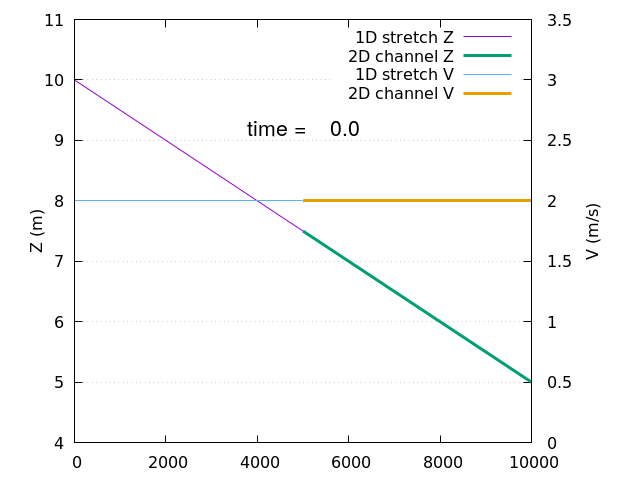
\includegraphics[width=0.45\textwidth]{figures/Channel_Manning_t=0.png}\label{fig:Channel_Maning_1}}
  ~
  \subfloat[coupled solution for R1 at t=180s]{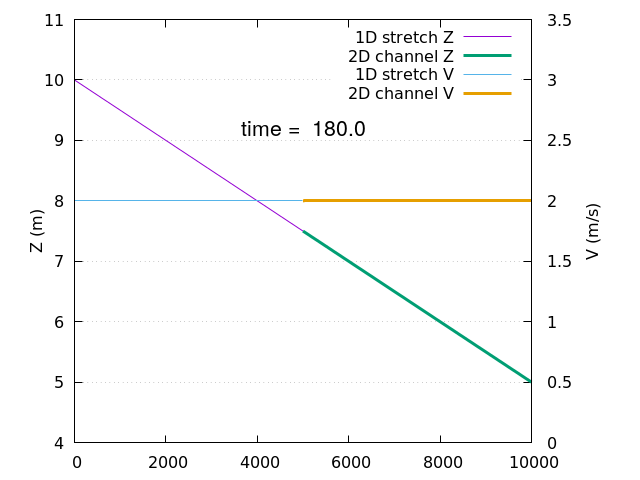
\includegraphics[width=0.45\textwidth]{figures/Channel_Manning_t=180.png}\label{fig:Channel_Manning_2}}
  \caption{1D-2D coupled solution for R1}\label{fig:Channel_Manning}
\end{figure}

\begin{figure}[htbp]
  \centering
  \subfloat[coupled solution for R2 at
    t=0s]{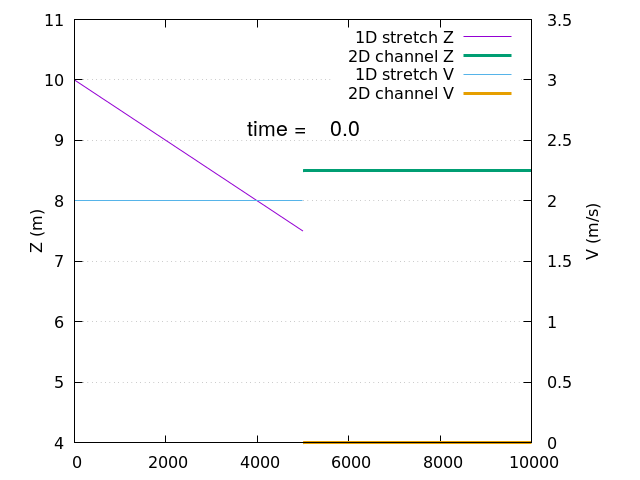
\includegraphics[width=0.45\textwidth]{figures/Channel_IC_t=0.png}\label{fig:Channel_1}}
  ~
  \subfloat[coupled solution for R2 at t=7180s]{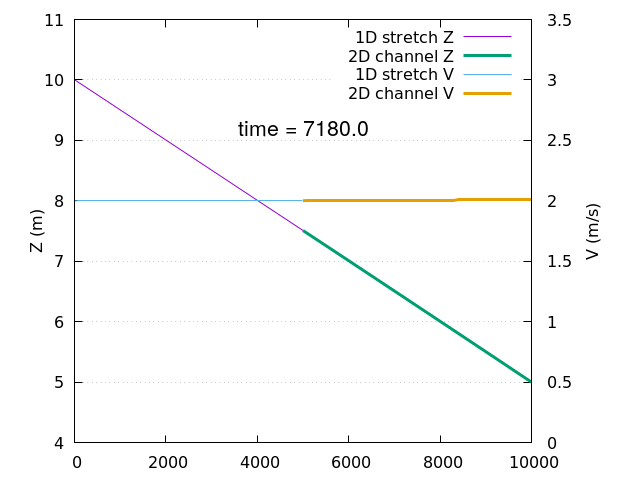
\includegraphics[width=0.45\textwidth]{figures/Channel_IC_t=7180.png}\label{fig:Channel_2}}
  \caption{1D-2D coupled solution for R2}\label{fig:Channel_IC}
\end{figure}

\begin{figure}[htbp]
  \centering
  \subfloat[coupled solution for R3 at t=0s]{ 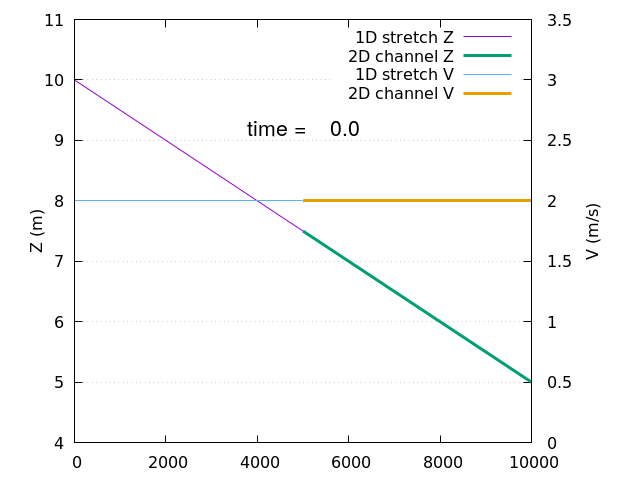
\includegraphics[width=0.45\textwidth]{figures/Channel_BC_t=0.png}\label{fig:Channel_Law_1}}
  ~
  \subfloat[coupled solution for R3 at t=500s]{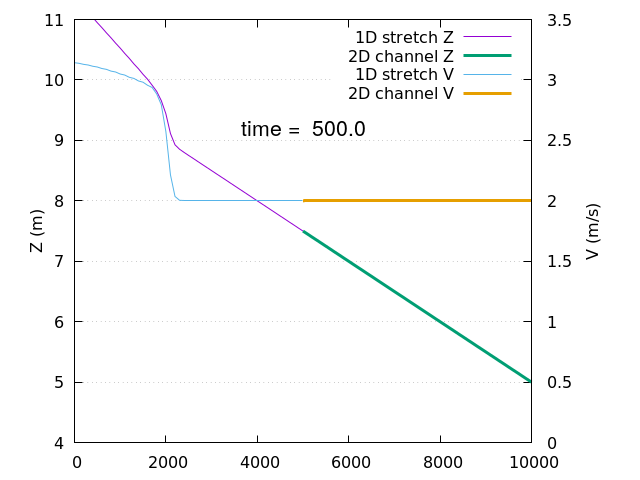
\includegraphics[width=0.45\textwidth]{figures/Channel_BC_t=500.png}\label{fig:Channel_Law_2}}
  \\
  \subfloat[coupled solution for R3 at t=1400s]{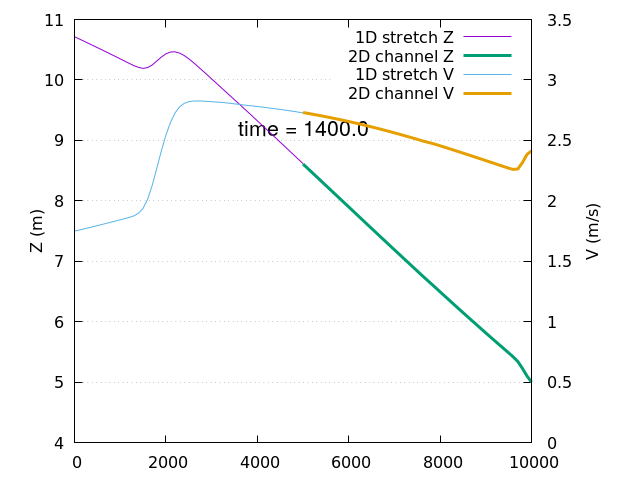
\includegraphics[width=0.45\textwidth]{figures/Channel_BC_t=1400.png}\label{fig:Channel_Law_3}}
  ~
  \subfloat[coupled solution for R3 at t=7180s]{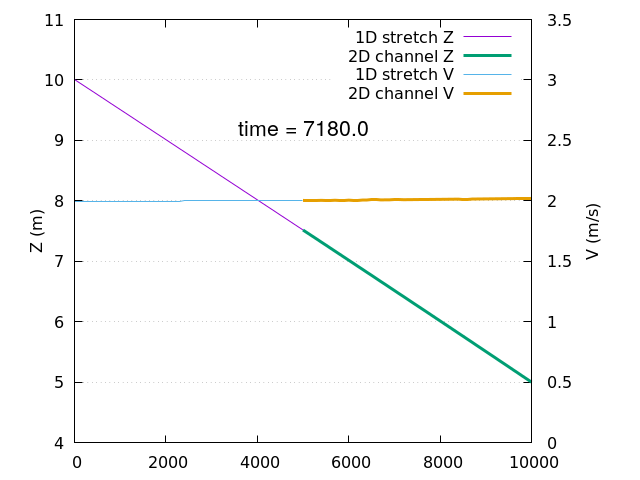
\includegraphics[width=0.45\textwidth]{figures/Channel_BC_t=7180.png}\label{fig:Channel_Law_4}}
  \caption{1D-2D coupled solution for R3}\label{fig:Channel_BC}
\end{figure}

\section{Adour catchment test case}
\subsection{Description of the test case and experiment settings}
The modelled domain is the confluence of the Nive and the Adour rivers
in Bayonne: the confluence is modeled with TELEMAC-2D and the upstream
Nive and Adour and the downstream Adour stretches are modeled with
MASCARET. For this case study, three 1D sub-domains are considered:
two 1D sud-domains represent the Nive and Adour rivers (respectively
Adour upstream and Nive upstream) that gather in the 2D domain, then
the Adour river is represented by a downstream 1D model (Adour
downstream) as illustrated in Fig.~\ref{fig:schema_coupling_2}. 

\subsection{Test case directory}
The test case files are in 
\texttt{examples/python3/telapy\_coupling/channel\_bayonne}.\\

The coupling is described as a user driven application and the
\texttt{driven\_coupling.py} procedure is provided in the test case
directory.\\
Notice that the procedure checks in the telemac configuration file if
the 2D model has been compiled with the \texttt{mpi} option and
trigger the \texttt{"Parallel"} option for \texttt{"Bayonne"} in the
\texttt{"2D"} section  \texttt{config\_run} dictionary accordingly.\\

The 1D and 2D model input files are organized as follows : 
\begin{itemize}
\item \texttt{/Input\_Data/RUN\_Adour\_amont} for the 1D model
  MASCARET on the upstream Adour strecth, containing, in turn, the
  \texttt{DonneesStat} directory containing the \texttt{.geo}, \texttt{.xcas},
  and \texttt{.lig} files for geometry, parameters and initial
  condition respectively and the \texttt{DonneesDyn} directory
  containing the \texttt{.loi} files for the boundary conditions.
\item \texttt{/Input\_Data/RUN\_Adour\_aval} for the 1D model
  MASCARET on the downstream Adour strecth, containing, in turn, the
  \texttt{DonneesStat} directory containing the \texttt{.geo}, \texttt{.xcas},
  and \texttt{.lig} files for geometry, parameters and initial
  condition respectively and the \texttt{DonneesDyn} directory
  containing the \texttt{.loi} files for the boundary conditions.
\item \texttt{/Input\_Data/RUN\_Nive\_amont} for the 1D model
  MASCARET on the upstream Nive strecth, containing, in turn, the
  \texttt{DonneesStat} directory containing the \texttt{.geo}, \texttt{.xcas},
  and \texttt{.lig} files for geometry, parameters and initial
  condition respectively and the \texttt{DonneesDyn} directory
  containing the \texttt{.loi} files for the boundary conditions.
\item \texttt{/Input\_Data/Bayonne} for the 2D model TELEMAC,
  containing the \texttt{TelemacBayonne.cas},\\
  \texttt{TelemacBayonne\_TypeDeConditionsLimites.cli},\\
  \texttt{TelemacBayonne\_ConditionsLimites.liq},\\ 
  \texttt{TelemacBayonne\_Geometrie\_Ks.slf} and\\
  \texttt{WaterLineInit\_43200.slf} files for parameters, 
  BC, parameters options, geometry and IC respectively. 
\end{itemize}

\subsection{Running the example}

The test case can be run as a user
driven application.\\

The user application driving the coupling is in the
\texttt{driven\_coupling.py} file. The launching procedure is:
\begin{verbatim}
cd $HOMETEL/examples/python3/telapy_coupling/channel_bayonne
python driven_coupling.py
\end{verbatim}
As such it is also part of the validation suite.

%%%%%%%%%%%%%%%%%%%%%%%%%%%%%%%%%%%%%%%%%%%%%%%%%%%%%%%%%%%%%%%%%%%%%%%%%


\begin{appendices}
  \chapter{Installation of the python venv}\label{ann:venv_install}

  You need to create a fresh virtual environment based on
  \texttt{python3} and to activate it.
  You have to provide a name for the dedicated
environment: in the following instructions we arbitrarily chose
\texttt{cpl\_py3}. The \texttt{VENVROOT} environment variable has to
be defined beforehands and point to the location on your machine where
the site packages will be installed. Make sure that there is enough
room avalaible and, in case of clusters with different
computational and front-end nodes, that the location can be accessed
from both kinds of nodes.
\begin{verbatim}
xxx>python3 -m venv $VENVROOT/cpl_py3

xxx>source $VENVROOT/cpl_py3/bin/activate
\end{verbatim}

If the virtual evironment has been correctly charged, the prompt will
be modified and display the active venv name. You can check that the
default \texttt{python} command now points to version 3.
\begin{verbatim}
(cpl_py3) xxx>python --version
Python 3.6.5
(cpl_py3) xxx>
\end{verbatim}

In order to access the most up to date view of the python packages we
suggest to upgrade the \texttt{pip} package manager itself to its latest
version
\begin{verbatim}
(cpl_py3) xxx>pip install --upgrade pip
\end{verbatim}

Since \texttt{pip} takes care of the dependencies, by installing a few
packages we have a complete environment that can be used for the
coupling, the data assimilation via Smurf and the Uncertainty
Quantification studies.
\begin{verbatim}
(cpl_py3) xxx>pip install ot-batman
(cpl_py3) xxx>pip install shapely
(cpl_py3) xxx>pip install pyyaml
\end{verbatim}

An optional package which can be useful if the user needs to determine
the number of physical cores (and not hyperthreaded processing units)
on his machine is \texttt{cpu\_cores}
\begin{verbatim}
(cpl_py3) xxx>pip install cpu_cores
\end{verbatim}

\section{Installation of mpi4py}\label{ann:venv_mpi4py}
The coupling communications being performed by MPI we need the
\texttt{mpi4py} package, but the installation has to be coherent with
the MPI flavour used for the compilation of telemac, if its parallel
version has been compiled.

Please, check that the commands \texttt{mpicc} and \texttt{mpirun}
found by default in your environment (as determined by the
\texttt{PATH} variable) are the same that you used to compile Open
TELEMAC-MASCARET.

In our case we check that
\begin{verbatim}
(cpl_py3) xxx>which mpicc
/softs/local/openmpi400_gcc731/bin/mpicc

(cpl_py3) xxx>mpicc --version
gcc (GCC) 7.3.1 20180130 (Red Hat 7.3.1-2)
\end{verbatim}
and
\begin{verbatim}
(cpl_py3) xxx>which mpirun
/softs/local/openmpi400_gcc731/bin/mpirun

(cpl_py3) xxx>mpirun --version
mpirun (Open MPI) 4.0.0
\end{verbatim}

Once the paths are correctly set, you can proceed to the installation
\begin{verbatim}
(cpl_py3) xxx>pip install mpi4py
\end{verbatim}


\chapter{Installation of the conda
  environment}\label{ann:conda_install}

If conda is not yet installed on your machine, please refer to
\url{https://www.anaconda.com/}

For a lighter installation, we suggest the use of miniconda3
[\url{https://docs.conda.io/en/latest/miniconda.html}].
\newline

You need to create a complete environment under python3 (the default
python version for miniconda3), but you should avoid to install
\texttt{mpi4py} from conda itself ({\em cf.} section
\ref{ann:mpi4py}). You have to provide a name for the dedicated
environment: in the following instructions we arbitrarily chose \texttt{cpl\_py3}.
\begin{verbatim}
xxx>source deactivate

xxx>conda update -n base conda

xxx>conda create -n cpl_py3 -c conda-forge \
>python openturns=1.10 matplotlib numpy pandas scipy scikit-learn \
>pathos jsonschema paramiko sphinx sphinx_rtd_theme pytest \
>pytest-runner mock ffmpeg shapely cython

xxx>source activate cpl_py3
\end{verbatim}


\section{Installation of mpi4py}\label{ann:mpi4py}
It is mandatory that the python MPI interface \texttt{mpi4py} is
compiled against the same version of MPI used for the coupled
codes. For this reason we should not install the precompiled version
provided by conda, but we have to compile and install it via
\texttt{pip}.
\newline

Please, check that the commands \texttt{mpicc} and \texttt{mpirun}
found by default in your environment (as determined by the
\texttt{PATH} variable) are the same that you used to compile Open
TELEMAC-MASCARET.

In our case we check that
\begin{verbatim}
xxx>which mpicc
/softs/local/openmpi400_gcc731/bin/mpicc

xxx>mpicc --version
gcc (GCC) 7.3.1 20180130 (Red Hat 7.3.1-2)
\end{verbatim}
and
\begin{verbatim}
xxx>which mpirun
/softs/local/openmpi400_gcc731/bin/mpirun

xxx>mpirun --version
mpirun (Open MPI) 4.0.0
\end{verbatim}

Once the paths are correctly set, you can proceed to the installation of
\texttt{mpi4py}.
Notice that the installation is normally driven by
\begin{verbatim}
xxx>pip install mpi4py
\end{verbatim}
but that a specific feature of OpenMPI 4 requires a maintenance
version, until the official mpi4py distro isn't updated
\begin{verbatim}
xxx>pip install --user https://bitbucket.org/mpi4py/mpi4py/get/maint.zip
\end{verbatim}

\chapter{A complete example of
  \texttt{coupling\_description.py}}\label{app:coupling_description}

Taken from
\begin{verbatim}
$HOMETEL/examples/python3/telapy_coupling/channel_manning/\
coupling_description.py
\end{verbatim}

\begin{verbatim}
coupling_def = {
    "Coupling": {
        "TimeStep": 10.0,
        "Method": "MultiplicativeSchwarz",
        "MaxIter": 5,
        "CplStepRestart1D": "Persist2D",
        "CplStepRestart2D": "Persist1D"
    },
    "1D": {
        "ch1d": {
            "TimeStep": 10.0,
            "OutputFreq": 10.0
        }
    },
    "2D": {
        "ch2d": {
            "TimeStep": 1.0,
            "OutputFreq": 10.0
        }
    },
    "Interfaces": [
        {
            "Id1D": "ch1d",
            "IdExtr1D": "downstream",
            "Condition1D": "Discharge",
            "Id2D": "ch2d",
            "LiqBdry2D": 2,
            "1DPosition": "UpStream",
            "ConvCriteria": {
                "Height": 0.01,
                "Velocity": 0.015
            }
        }
    ]
}

config_run = {
    "Run": {
        "RefDate": "1/1/2019 00:00:00",
        "StartDate": "1/1/2019 00:00:00",
        "EndDate": "1/1/2019 00:03:20",
        "SingleExecDuration": "00:01:40",
        "RestartFromFile": "yes"
    },
    "2D": {
        "ch2d": {
            "Parallel": "no",
            "NbProc": 4
        }
    }
}

config_ch1d = {
    "files": {

        "xcas": "../Input_Data/1d_stretch/ParametresMascaret.xcas",
        "geo": "../Input_Data/1d_stretch/Channel1d.geo",
        "res": "ResultatsOpthyca_ch1d.opt",
        "listing": "ResultatsListing_ch1d.lis",
        "damocle": "listing.damoc",
        "lig": "../Input_Data/1d_stretch/WaterLine_ch1d.lig",
        "loi": [
            "../Input_Data/1d_stretch/1d_up.loi",
            "../Input_Data/1d_stretch/1d_down.loi"
        ]
    }
}
config_ch2d = {
    "files": {
        "cas": "../Input_Data/2d_rect/T2DCAS"
    }
}
\end{verbatim}

\chapter{A complete example of user defined
  procedure}\label{app:driven_coupling}

Taken from
\begin{verbatim}
$HOMETEL/examples/python3/telapy_coupling/channel_manning/\
driven_coupling.py
\end{verbatim}
Notice that, w.r.t. to the run configuration for the same case
described in App. \ref{app:coupling_description}, in this example the
two single executions are run via two calls to the driver with two
different \texttt{config\_run} dictionaries.

\begin{verbatim}
import os
from telapy.coupling.long_cpl_driver import LongCplDriver

user_coupling = {
    "Coupling": {
        "TimeStep": 10.0,
        "Method": "MultiplicativeSchwarz",
        "MaxIter": 5,
        "CplStepRestart1D": "Persist2D",
        "CplStepRestart2D": "Persist1D"
    },
    "1D": {
        "ch1d": {
            "TimeStep": 10.0,
            "OutputFreq": 10.0
        }
    },
    "2D": {
        "ch2d": {
            "TimeStep": 1.0,
            "OutputFreq": 10.0
        }
    },
    "Interfaces": [
        {
            "Id1D": "ch1d",
            "IdExtr1D": "downstream",
            "Condition1D": "Discharge",
            "Id2D": "ch2d",
            "LiqBdry2D": 2,
            "1DPosition": "UpStream",
            "ConvCriteria": {
                "Height": 0.01,
                "Velocity": 0.015
            }
        }
    ]
}

models_configs = {
    "config_ch1d" : {
        "files": {

            "xcas": "../Input_Data/1d_stretch/ParametresMascaret.xcas",
            "geo": "../Input_Data/1d_stretch/Channel1d.geo",
            "res": "ResultatsOpthyca_ch1d.opt",
            "listing": "ResultatsListing_ch1d.lis",
            "damocle": "listing.damoc",
            "lig": "../Input_Data/1d_stretch/WaterLine_ch1d.lig",
            "loi": [
                "../Input_Data/1d_stretch/1d_up.loi",
                "../Input_Data/1d_stretch/1d_down.loi"
            ]
        }
    },
    "config_ch2d" : {
        "files": {
            "cas": "../Input_Data/2d_rect/T2DCAS"
        }
    }
}


driven_run = {
    "Run": {
        "RefDate": "1/1/2019 00:00:00",
        "StartDate": "1/1/2019 00:00:00",
        "EndDate": "1/1/2019 00:01:40",
        "SingleExecDuration": "00:01:40",
        "RestartFromFile": "yes"
    },
    "2D": {
        "ch2d": {
            "Parallel": "no",
            "NbProc": 4
        }
    }
}

the_coupling = LongCplDriver(".", user_coupling, models_configs)
the_coupling(driven_run)

driven_run["Run"]["StartDate"] = driven_run["Run"]["EndDate"]
driven_run["Run"]["EndDate"] = "1/1/2019 00:03:20"
the_coupling(driven_run)
\end{verbatim}

\chapter{A complete example of json input files}

This example translates into json files the configuration of\\
\texttt{\$HOMETEL/examples/python3/telapy\_coupling/channel\_ic}

\section{A complete example of
  \texttt{CouplingDef.json}}\label{app:CouplingDef}

\begin{verbatim}
{
    "Coupling" : {
        "TimeStep" : 10.0,
        "Method" : "MultiplicativeSchwarz",    
        "MaxIter"  : 5,
        "CplStepRestart1D" : "Persist2D",
        "CplStepRestart2D" : "Persist1D"
    },
    "1D" : {
        "ch1d" : {
            "TimeStep" : 10.0,
            "OutputFreq" : 20.0
        }
    },
    "2D" : {
        "ch2d" : {
            "TimeStep" : 1.0,
            "OutputFreq" : 20.0,
            "OutputSites" : [18, 33, 1018, 1024, 1034, 1044, 1054,
                             1064, 1074, 1084, 1094, 1104,
                             1114, 1124, 1134, 1144, 1154,
                             1164, 1174, 1184, 1194, 1204,
                             1214, 1224, 1234, 1244, 1254,
                             1264, 1274, 1284, 1294, 1304,
                             1314, 1324, 1334, 1344, 1354,
                             1364, 1374, 1384, 1394, 1404,
                             1414, 1424, 1434, 1444, 1454,
                             1464, 1474, 1484, 1494, 1504,
                             30]
        }
    },
    "Interfaces" : [
        {
            "Id1D" : "ch1d",
            "IdExtr1D" : "downstream",
            "Condition1D" : "Discharge",
            "Id2D" : "ch2d",
            "LiqBdry2D" : 2,
            "1DPosition" : "UpStream",
            "ConvCriteria" : {
                "Height" : 0.01,
                "Velocity" : 0.015
            }
        }
    ]
}
\end{verbatim}

\section{A complete example of
  \texttt{ConfigRun.json}}\label{app:ConfigRun}

\begin{verbatim}
{
    "Run" : {
        "RefDate" : "1/1/2019 00:00:00",
        "StartDate" : "1/1/2019 00:00:00",
        "EndDate"   : "1/1/2019 02:00:00",
        "SingleExecDuration" : "02:00:00",
        "RestartFromFile" : "no"
    },
    "2D" : {
        "ch2d" : {
            "Parallel" : "no",
            "NbProc" : 4
        }
    }
}
\end{verbatim}

\section{A complete example of
  \texttt{config\_ch1d.json}}\label{app:config_ch1d}

\begin{verbatim}
{
 "files": {
        "xcas": "../Input_Data/1d_stretch/ParametresMascaret.xcas",
        "geo": "../Input_Data/1d_stretch/Channel1d.geo",
        "res": "ResultatsOpthyca_ch1d.opt",
        "listing": "ResultatsListing_ch1d.lis",
        "damocle": "listing.damoc",
        "lig": "../Input_Data/1d_stretch/WaterLine_ch1d.lig",
        "loi": [
                "../Input_Data/1d_stretch/1d_up.loi",
                "../Input_Data/1d_stretch/1d_down.loi"
               ]
        }
}
\end{verbatim}

\section{A complete example of
  \texttt{config\_ch2d.json}}\label{app:config_ch2d}

\begin{verbatim}
{
 "files": {
        "config_file" : "${SYSTELCFG}",
        "config_option" : "${USETELCFG}",
        "cas" : "../Input_Data/2d_rect/T2DCAS"
        }
}
\end{verbatim}

\end{appendices}

%\scriptsize
\bibliographystyle{plainnat}   
\bibliography{coupling_user.bib}

\end{document}
